% Created 2022-02-22 Di 14:22
% Intended LaTeX compiler: pdflatex
\documentclass[presentation]{beamer}
\usepackage[utf8]{inputenc}
\usepackage[T1]{fontenc}
\usepackage{graphicx}
\usepackage{grffile}
\usepackage{longtable}
\usepackage{wrapfig}
\usepackage{rotating}
\usepackage[normalem]{ulem}
\usepackage{amsmath}
\usepackage{textcomp}
\usepackage{amssymb}
\usepackage{capt-of}
\usepackage{hyperref}
\usepackage{minted}
\usepackage[utf8]{inputenc}
\usepackage{color}
\usetheme[height=7mm]{Rochester}
\setbeamertemplate{footline}[frame number]
\usecolortheme[accent=red, light]{solarized}
\setbeamercolor{frametitle}{bg=solarizedRebase02,fg=solarizedAccent}
\setbeamercolor{author in head/foot}{bg=solarizedRebase02,fg=solarizedRebase01}
\setbeamercolor{title in head/foot}{bg=solarizedRebase02,fg=solarizedRebase01}
\setbeamercolor{block title}{bg=solarizedRebase0,fg=solarizedRebase02}
\setbeamercolor{block body}{bg=solarizedRebase02,fg=solarizedRebase0}
\setbeamercolor{item}{bg=solarizedRebase02,fg=solarizedAccent}
\beamertemplatenavigationsymbolsempty
\usemintedstyle{manni}
\AtBeginSection[]{
\begin{frame}
\vfill
\centering
\begin{beamercolorbox}[sep=8pt,center,shadow=true,rounded=true]{title}
\Huge\insertsectionhead\par%
\end{beamercolorbox}
\vfill
\end{frame}
}
\usetheme{default}
\author{Thomas Hausberger, Matthias Panny \\ Ursprünglich erstellt von Sebastian Stabinger}
\date{SS2022}
\title{Einführung in C++: Strings, Vektoren, \ldots{}}
\hypersetup{
 pdfauthor={Thomas Hausberger, Matthias Panny \\ Ursprünglich erstellt von Sebastian Stabinger},
 pdftitle={Einführung in C++: Strings, Vektoren, \ldots{}},
 pdfkeywords={},
 pdfsubject={},
 pdfcreator={Emacs 27.2 (Org mode 9.4.4)}, 
 pdflang={Ger}}
\begin{document}

\maketitle

\section{Strings}
\label{sec:org34863a6}
\begin{frame}[label={sec:orgbbff279},fragile]{Strings in C}
 \begin{itemize}
\item Ein Array vom Typ {\color{solarizedYellow}\verb!char!}
\item Wir müssen uns selbst um die Größe kümmern
\item Ende des Strings ist durch das Zeichen {\color{solarizedYellow}\verb!\0!} gekennzeichnet
\end{itemize}
\begin{block}{Beispiel für einen C String im Speicher}
\begin{minted}[numberblanklines=false,fontsize=\scriptsize]{c++}
char str[] = "PROGRAM";
\end{minted}
\begin{center}
\includegraphics[width=.9\linewidth]{data/cb/fcc991-bddd-49c7-a9fb-fff24aa41a8b/screenshot-20160221-203103.png}
\end{center}
\end{block}
\end{frame}
\begin{frame}[label={sec:orgcf6e780},fragile]{Strings in C: Ein Beispiel}
 Wir wollen den Inhalt von zwei Strings {\color{solarizedYellow}\verb!str1!} und {\color{solarizedYellow}\verb!str2!}
aneinanderhängen und das Ergebnis in {\color{solarizedYellow}\verb!str3!} speichern.
\begin{exampleblock}{Beispiel}
\begin{minted}[numberblanklines=false,fontsize=\scriptsize]{c}
#include <stdio.h>
#include <string.h>

// Wir müssen uns selbst darum kümmern, dass str3 groß genug ist
char str1[100], str2[100], str3[200];
strcpy(str1, "Hello ");
// str1 = "Hello " funktioniert nicht!
strcpy(str2, "World");
// Hänge str1 und str2 zusammen und speichere in str3
strcpy(str3, str1);
strcat(str3, str2);
// Gib str3 auf Bildschirm aus
printf("%s", str3);  // Wir müssen den Typ von str3 angeben (%s)
\end{minted}
\end{exampleblock}
Man sieht: Die Verwendung ist \alert{umständlich und unnatürlich}
\end{frame}
\begin{frame}[label={sec:org132888b},fragile]{Strings in C++}
 \begin{itemize}
\item Ein eigener Datentyp names {\color{solarizedYellow}\verb!std::string!}
\item Die Größe wird dynamisch angepasst
\item Verhält sich wie man es erwarten würde!
\end{itemize}
\begin{exampleblock}{Beispiel}
\begin{minted}[numberblanklines=false,fontsize=\scriptsize]{c++}
#include <iostream>
#include <string>
using namespace std;

string str1, str2, str3; // Platz für beliebig viele Zeichen
str1 = "Hello ";         // Wir können einfach zuweisen
str2 = "World";
// Hänge str1 und str2 zusammen und speichere in str3
str3 = str1 + str2;
// Gib str3 auf Bildschirm aus
cout << str3 << endl; // Der Compiler kennt den Typ!
\end{minted}
\end{exampleblock}
\begin{itemize}
\item Falls wir z.B. {\color{solarizedYellow}\verb!str3!} als C-String benötigen:  {\color{solarizedYellow}\verb!str3.c_str()!}
\end{itemize}
\end{frame}
\begin{frame}[label={sec:org7c6a322},fragile]{Vergleichen von Strings}
 Um zu testen, ob zwei Strings gleich sind muss in C eine spezielle
Funktion ({\color{solarizedYellow}\verb!strcmp!}) verwendet werden. In C++ erfolgt der Vergleich
ganz natürlich mit dem Vergleichsoperator {\color{solarizedYellow}\verb!==!}, wie bei allen anderen
Datentypen auch.
\begin{exampleblock}{C}
\begin{minted}[numberblanklines=false,fontsize=\scriptsize]{c}
if (strcmp(str1, str2) == 0) {
  printf("String 1 und 2 sind gleich");
}
\end{minted}
\end{exampleblock}
\begin{exampleblock}{C++}
\begin{minted}[numberblanklines=false,fontsize=\scriptsize]{c++}
if (str1 == str2) {
  std::cout << "String 1 und 2 sind gleich";
}
\end{minted}
\end{exampleblock}
\end{frame}
\begin{frame}[label={sec:org54cfb21},fragile]{Konvertierungen}
 \begin{block}{\ldots{} in einen String}
Zahlen können mittels der Funktion {\color{solarizedYellow}\verb!to_string!} in einen {\color{solarizedYellow}\verb!string!}
konvertiert werden.
\begin{minted}[numberblanklines=false,fontsize=\scriptsize]{c++}
string s = to_string(42);  // s enthält den String "42"
\end{minted}
\end{block}
\begin{block}{\ldots{} von einem String}
Ein String welcher eine Zahl enthält kann mit folgenden Funktionen in
eine Zahl konvertiert werden:
\begin{itemize}
\item {\color{solarizedYellow}\verb!stoi!}, {\color{solarizedYellow}\verb!stol!}, {\color{solarizedYellow}\verb!stoll!} für Integer, Long und Long Long
\item {\color{solarizedYellow}\verb!stof!}, {\color{solarizedYellow}\verb!stod!}, {\color{solarizedYellow}\verb!stold!} für Float, Double und Long Double
\end{itemize}
\begin{minted}[numberblanklines=false,fontsize=\scriptsize]{c++}
int i = stoi("42"); // i enthält die Zahl 42
\end{minted}
\end{block}
Für komplexere Umwandlungen verwendet man einen {\color{solarizedYellow}\verb!stringstream!}.
\end{frame}
\begin{frame}[label={sec:org2eb3d10},fragile]{Daten formatieren mit {\color{solarizedYellow}\texttt{stringstream}} [optional]}
 \begin{itemize}
\item Man erzeugt einen \alert{String Stream} mittels {\color{solarizedYellow}\verb!stringstream!} (benötigt
{\color{solarizedYellow}\verb!sstream!} als Include)
\item Schreiben wie in {\color{solarizedYellow}\verb!cout!}
\item Um daraus einen String zu erzeugen: {\color{solarizedYellow}\verb!.str()!}
\end{itemize}
\begin{exampleblock}{Beispiel}
\begin{minted}[numberblanklines=false,fontsize=\scriptsize]{c++}
#include <iostream>
#include <sstream>
using namespace std;

int main() {
  stringstream str_stream;
  str_stream << "Die Antwort ist " << 42 << " !";
  string str = str_stream.str();

  cout << str << endl;
} // Ausgabe: Die Antwort ist 42 !
\end{minted}
\end{exampleblock}
\end{frame}
\begin{frame}[label={sec:orgd384447},fragile]{Daten extrahieren mit {\color{solarizedYellow}\texttt{stringstream}} [optional]}
 \begin{itemize}
\item {\color{solarizedYellow}\verb!stringstream ss(string)!} erzeugt einen Stringstream namens {\color{solarizedYellow}\verb!ss!} aus
einem bereits existierenden String.
\item Aus einem {\color{solarizedYellow}\verb!stringstream!} können wie mittels {\color{solarizedYellow}\verb!cin!} Daten ausgelesen
werden
\end{itemize}
\begin{exampleblock}{Beispiel}
\begin{minted}[numberblanklines=false,fontsize=\scriptsize]{c++}
#include <iostream>
#include <sstream>
#include <string>
using namespace std;

int main() {
  string s = "23 42 47";
  stringstream str_stream(s); // oder direkt str_stream("23 42 47")
  int a, b, c;
  str_stream >> a >> b >> c; // Einlesen der Daten

  cout << "a=" << a << " b=" << b << " c=" << c << endl;
} // Ausgabe: a=23 b=42 c=47
\end{minted}
\end{exampleblock}
\end{frame}

\section{\texttt{vector} als Array-Alternative}
\label{sec:org45cae57}
\begin{frame}[label={sec:org049c69f},fragile]{Fundamentale Arrays --- Einige Probleme}
 \begin{block}{Größe ist nicht Teil des Datentyps}
\begin{minted}[numberblanklines=false,fontsize=\scriptsize]{c++}
int sum(int *a, int length) {
  // Länge muss explizit mitgegeben werden
  int sum = 0;
  for (int i = 0; i < length; i++) {
    sum += a[i];
  }
  return sum;
}
\end{minted}
\end{block}
\begin{block}{Keine Überprüfung von Indexfehlern}
\begin{minted}[numberblanklines=false,fontsize=\scriptsize]{c++}
int a[10];
a[20] = 47; // Ouch! Kein Fehler!!
\end{minted}
\end{block}
\begin{itemize}
\item Die Größe muss vorab bekannt sein wenn man nicht dynamische
Speicherverwaltung verwenden will!
\end{itemize}
\end{frame}
\begin{frame}[label={sec:org644f764},fragile]{{\color{solarizedYellow}\texttt{vector}} --- Die C++ Alternative}
 Verwendbar mittels {\color{solarizedYellow}\verb!#include <vector>!}

Vorteile:
\begin{itemize}
\item Automatisches Speichermanagement
\item Dynamische Größe
\item Überprüft auf Indexfehler (wenn man das will)
\item Bietet viele komfortable Funktionen
\end{itemize}
\begin{exampleblock}{Arraybeispiel mit {\color{solarizedYellow}\texttt{vector}} implementiert}
\begin{minted}[numberblanklines=false,fontsize=\scriptsize]{c++}
vector<int> a(100); // Vektor mit Platz für 100 Integer Werte
// Vektor mit den Zahlen 1 bis 5
vector<int> b = {1, 2, 3, 4, 5};
// Ausgabe des ersten Elements von a und fünften von b
cout << "a[0]=" << a[0] << " b[4]=" << b[4] << endl;
// Ausgabe: a[0]=0 b[4]=5
\end{minted}
\end{exampleblock}
\end{frame}
\begin{frame}[label={sec:org8db7f41},fragile]{{\color{solarizedYellow}\texttt{vector}} mit bekannter Größe}
 Ein Vektor mit bekannter Größe kann folgendermaßen deklariert werden: {\color{solarizedYellow}\verb!vector<typ> name(größe);!}
\begin{exampleblock}{Beispiel}
\begin{minted}[numberblanklines=false,fontsize=\scriptsize]{c++}
vector<int> a(100); vector<double> bla(400);
\end{minted}
\end{exampleblock}
Im Gegensatz zu einem Fundamentalen Array kann die Größe aber auch
erst \alert{zur Laufzeit} festgelegt werden. D.h. \alert{als Größe kann auch eine
Variable} angegeben werden (in C seit C99 auch möglich) und die
\alert{Größe} kann problemlos \alert{zur Laufzeit verändert werden}.
\begin{exampleblock}{Beispiel}
Angenommen {\color{solarizedYellow}\verb!get_num!} fragt den Benutzer nach einer Zahl und gibt
diese zurück
\begin{minted}[numberblanklines=false,fontsize=\scriptsize]{c++}
int size = get_num();
vector<int> vec(size);
// vec hat die Größe welche der Benutzer eingegeben hat
\end{minted}
\end{exampleblock}
\end{frame}
\begin{frame}[label={sec:org0110265},fragile]{Der leere Vektor}
 Für die Verwendung von {\color{solarizedYellow}\verb!vector!} muss die benötigte \alert{Größe nicht von
Anfang an bekannt sein}. Wir lassen die Größe einfach weg und erzeugen
damit einen leeren Vektor: {\color{solarizedYellow}\verb!vector<typ> name;!}
\begin{exampleblock}{Beispiel}
\begin{minted}[numberblanklines=false,fontsize=\scriptsize]{c++}
vector<int> a; vector<double> bla;
\end{minted}
\end{exampleblock}
\begin{alertblock}{Vorsicht!}
Sie dürfen nicht auf Elemente eines Vektors zugreifen wenn diese nicht
existieren!
\begin{minted}[numberblanklines=false,fontsize=\scriptsize]{c++}
vector<int> a; // Vektor hat Größe 0
a[0] = 10; // Im besten Fall ein Speicherfehler ...
cout << a[0] << endl; // ... im ungünstigsten Fall unvorhersehbar
\end{minted}
\end{alertblock}
\end{frame}
\begin{frame}[label={sec:org696c5fb},fragile]{Wofür ein leerer Vektor?}
 Wenn man nicht auf Elemente eines leeren Vektors zugreifen kann, wofür
ist er dann nützlich?
\begin{exampleblock}{Späteres Festlegen der Größe mit {\color{solarizedYellow}\texttt{resize}}}
\begin{minted}[numberblanklines=false,fontsize=\scriptsize]{c++}
vector<int> a;
a.resize(100); // Vektor a hat jetzt Platz für 100 Integer
a.resize(200); // Vektor a hat jetzt Platz für 200 Integer
\end{minted}
\end{exampleblock}
\begin{exampleblock}{Anhängen von Elementen mit {\color{solarizedYellow}\texttt{push_back}}}
\begin{minted}[numberblanklines=false,fontsize=\scriptsize]{c++}
vector<int> a;
a.push_back(12);
a.push_back(23);
a.push_back(42);
// a enthält nun {12, 23, 42}
\end{minted}
\end{exampleblock}
\end{frame}
\begin{frame}[label={sec:org47f9082},fragile]{Zugriff auf Elemente}
 \begin{minted}[numberblanklines=false,fontsize=\scriptsize]{c++}
vector<int> vec;
vec.push_back(23); vec.push_back(42); vec.push_back(7);
\end{minted}
\begin{block}{Ohne Bounds Checking (schneller)}
Funktioniert wie bei Arrays mittels {\color{solarizedYellow}\verb![index]!}
\begin{minted}[numberblanklines=false,fontsize=\scriptsize]{c++}
vec[0]; // == 23
vec[2]; // == 7
vec[5]; // == ?? keinerlei Garantien
\end{minted}
\tiny VisualStudio macht bei Debug Builds auch hier ein Bounds
Checking! Kann bei den meinsten Compilern eingestellt werden (z.B. für
gcc mit dem Compilerflag {\color{solarizedYellow}\verb!-D_GLIBCXX_DEBUG!})
\end{block}
\begin{block}{Mit Bounds Checking (sicherer)}
Mit Hilfe der Funktion {\color{solarizedYellow}\verb!.at(index)!}
\begin{minted}[numberblanklines=false,fontsize=\scriptsize]{c++}
vec.at(0); // == 23
vec.at(2); // == 7
vec.at(5); // Wirft zur Laufzeit zuverlässig eine Exception
\end{minted}
\end{block}
Beide Versionen können auch für die Zuweisung von Werten verwendet
werden: {\color{solarizedYellow}\verb!vec[1] = 10;!} bzw. {\color{solarizedYellow}\verb!vec.at(1) = 10;!}
\end{frame}
\begin{frame}[label={sec:org231b652},fragile]{Löschen von Elementen}
 \begin{itemize}
\item Es ist möglich \alert{einzelne Elemente} aus einem Vektor mit folgender
Funktion zu \alert{löschen}:
\end{itemize}
{\color{solarizedYellow}\verb!vektorname.erase(vektorname.begin() + position)!}
\begin{itemize}
\item Falls ein anderes Element als das letzte im Vektor gelöscht wird ist
die Operation \alert{relativ langsam} ({\color{solarizedYellow}\verb!list!} ist für solche Fälle eine
bessere Alternative zu {\color{solarizedYellow}\verb!vector!})
\item In den allermeisten Fällen aber trotzdem \alert{schnell genug}!
\end{itemize}
\end{frame}

\begin{frame}[label={sec:orgf6a03cd},fragile]{Löschen von Elementen --- Beispiel}
 \begin{block}{Beispiel}
\begin{minted}[numberblanklines=false,fontsize=\scriptsize]{c++}
#include <iostream>
#include <vector>
using namespace std;

int main() {
  vector<int> vec = {2, 6, 1, 28, 42, 23, 47, 7};

  vec.erase(vec.begin() + 3);

  for (int &i : vec)
    cout << i << " ";
}
\end{minted}
\end{block}

\begin{block}{Ausgabe}
\begin{verbatim}
2 6 1 42 23 47 7
\end{verbatim}
\end{block}
\end{frame}

\begin{frame}[label={sec:orgb91970c},fragile]{Weitere Nützliche Funktionen}
 \begin{itemize}
\item {\color{solarizedYellow}\verb!.size()!} Gibt die Anzahl an Elementen zurück
\item {\color{solarizedYellow}\verb!.empty()!} Gibt {\color{solarizedYellow}\verb!true!} zurück falls der Vektor keine Elemente enthält
\item {\color{solarizedYellow}\verb!.data()!} Gibt ein C-Array auf die Daten des Vektors zurück. Wichtig
falls man mit C-Code interagieren muss.
\item {\color{solarizedYellow}\verb!.pop_back()!} Löscht das letzte Element vom Vektor. Gegenstück zu
{\color{solarizedYellow}\verb!.push_back(element)!}.
\item {\color{solarizedYellow}\verb!.back()!} Gibt letztes Element des Vektors zurück ohne es zu löschen
\item {\color{solarizedYellow}\verb!==!} Zwei Vektoren können mittels {\color{solarizedYellow}\verb!==!} verglichen werden. Die
Vektoren gelten als gleich falls sie die gleiche Größe haben und die
selben Elemente enthalten. {\color{solarizedYellow}\verb!if(vec1 == vec2);!}
\end{itemize}
\end{frame}
\begin{frame}[label={sec:org6dbce1a},fragile]{Vector --- Beispiel}
 \begin{minted}[numberblanklines=false,fontsize=\scriptsize]{c++}
#include <iostream>
#include <vector>
using namespace std;

int main() {
  vector<int> vec;
  cout << "Größe von vec: " << vec.size() << endl;
  vec.push_back(23);
  vec.push_back(13);
  vec.push_back(42);
  vec.push_back(7);
  cout << "Größe von vec: " << vec.size() << endl;
  // For-each 
  for (auto e : vec)
    cout << e << " ";
}
\end{minted}
\begin{block}{Ausgabe}
\begin{minted}[numberblanklines=false,fontsize=\scriptsize]{text}
Größe von vec: 0
Größe von vec: 4
23 13 42 7 
\end{minted}
\end{block}
\end{frame}
\section{for-each}
\label{sec:orgc90ddb7}
\begin{frame}[label={sec:org40d78e0},fragile]{{\color{solarizedYellow}\texttt{for}} - each (neu in C++11)}
 Iteriert automatisch über alle Elemente eines "Containers" z.B. Array,
Vector, etc.
\begin{block}{Beispiel}
\begin{minted}[numberblanklines=false,fontsize=\scriptsize]{c++}
std::vector<int> vec = {23, 12, 42, 13, -40}; // Ein Array

for (int i : vec) {
  std::cout << i << " ";
}
\end{minted}
\end{block}
\begin{block}{Ausgabe}
\begin{verbatim}
23 12 42 13 -40
\end{verbatim}
\end{block}
\end{frame}
\begin{frame}[label={sec:org7d08b55},fragile]{{\color{solarizedYellow}\texttt{for}} - each --- Zuweisung}
 Um in einer for-each Schleife Werte in ein Array zu schreiben, muss
der Laufvariable ein {\color{solarizedYellow}\verb!&!} vorangestellt werden. Dies kennzeichnet die
Variable als eine sogenannte \alert{Referenz} (eine Alternative zu Zeigern
in C++)
\begin{block}{Beispiel 1}
\begin{minted}[numberblanklines=false,fontsize=\scriptsize]{c++}
std::vector<int> vec(100); // Ein Array der Größe 100

// Wir füllen das ganze Array mit dem Wert 23
for (int &i : vec) {
  i = 23;
}
\end{minted}
\end{block}
\end{frame}
\begin{frame}[label={sec:orga0f7a65},fragile]{{\color{solarizedYellow}\texttt{for}} - each --- Zuweisung}
 \begin{block}{Beispiel 2}
\begin{minted}[numberblanklines=false,fontsize=\scriptsize]{c++}
std::vector<int> vec = {1, 2, 3, 4, 5, 6, 7, 8, 9, 10};

// Quadriert alle Einträge in arr
for (int &i : vec) {
  i = i * i;
}

for (int i : vec) {
  std::cout << i << " ";
}
\end{minted}

\begin{verbatim}
1 4 9 16 25 36 49 64 81 100
\end{verbatim}
\end{block}
\end{frame}
\section{Funktionsüberladung}
\label{sec:org390ce43}
\begin{frame}[label={sec:org1f59737},fragile]{Funktionsüberladung}
 \begin{itemize}
\item Es können mehrere Funktionen mit \alert{gleichem Namen} deklariert werden
so lange die \alert{Datentypen der Argumente eindeutig} sind
\item Der \alert{Compiler wählt die korrekte Funktion} anhand der Datentypen der
an die Funktion übergebenen Argumente aus
\end{itemize}
\begin{block}{OK}
\begin{minted}[numberblanklines=false,fontsize=\scriptsize]{c++}
int f(int a);
double f(double a);
int f(short a);
int f(int a, int b); // Parameteranzahl ist auch wichtig
\end{minted}
\end{block}
\begin{block}{Fehlerhaft}
\begin{minted}[numberblanklines=false,fontsize=\scriptsize]{c++}
int f(int a);
int f(int b); // Error: nur der Typ zählt
double f(int a); // Error: Der Rückgabetyp wird ignoriert
\end{minted}
\end{block}
\end{frame}
\begin{frame}[label={sec:org1189eac},fragile]{Funktionsüberladung --- Beispiel}
 \begin{minted}[numberblanklines=false,fontsize=\scriptsize]{c++}
#include <iostream>

// int wird quadriert
int f(int a) { return a * a; }
// Bei double wird 10 hinzugezählt
double f(double a) { return a + 10; }
// short wird verdoppelt
short f(short a) { return a * 2; }

int main() {
  int a = 5;
  double b = 10;
  short c = 4;

  std::cout << "int: " << f(a) << " ";
  std::cout << "double: " << f(b) << " ";
  std::cout << "short: " << f(c) << " ";
}
\end{minted}
\begin{block}{Ausgabe}
\begin{minted}[numberblanklines=false,fontsize=\scriptsize]{text}
int: 25 double: 20 short: 8
\end{minted}
\end{block}
\end{frame}
\section{\texttt{auto}}
\label{sec:org6288ac0}
\begin{frame}[label={sec:orge4f499c},fragile]{{\color{solarizedYellow}\texttt{auto}} (neu in C++11)}
 \begin{itemize}
\item Seit C++11 unterstützt C++ eine einfache Form der sogenannten
\alert{Typinferenz} \footnote{\href{https://de.wikipedia.org/wiki/Typinferenz}{https://de.wikipedia.org/wiki/Typinferenz}}
\item Bedeutet: Falls der Compiler den Typ einer Variable selbst
herausfinden kann, muss man ihn nicht angeben.
\item Um Typinferenz zu verwenden schreibt man {\color{solarizedYellow}\verb!auto!} statt des
eigentlichen Datentyps.
\end{itemize}
\begin{block}{Beispiel}
\begin{minted}[numberblanklines=false,fontsize=\scriptsize]{c++}
auto i = 10;    // i ist vom Typ int
auto tmp = f(); // tmp hat den Typ welcher von f
		// zurückgegeben wird
\end{minted}
\end{block}
\end{frame}

\section{Zeiger}
\label{sec:org5f111d1}
\begin{frame}[label={sec:org6c33a77}]{Zeiger in C}
\begin{itemize}
\item Zeiger sind Variablen welche Adressen speichern können (also
normalerweise 64bit Integer)
\item Zeiger haben einen Typ
\begin{itemize}
\item Der Typ eines Zeigers gibt an, was an der Adresse auf die gezeigt
wird gespeichert ist.
\item Im Zeiger selbst wird unabhängig vom Typ immer das gleiche
gespeichert (eine Adresse)
\end{itemize}
\end{itemize}
\begin{center}
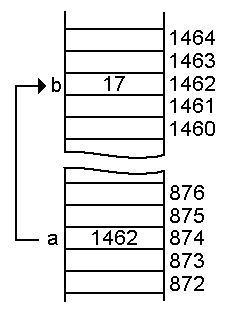
\includegraphics[width=0.3\textwidth]{img/pointer.png}
\end{center}
\end{frame}
\begin{frame}[label={sec:org9c337c3},fragile]{Beispiel und Probleme}
 \begin{block}{Beispiel}
\begin{minted}[numberblanklines=false,fontsize=\scriptsize]{c++}
int intVar = 10;
int *intPtr = &intVar;
cout << intVar << endl;
cout << *intPtr << endl;
intVar = 20;
cout << *intPtr << endl;
\end{minted}
\end{block}
\begin{block}{Probleme}
\begin{minted}[numberblanklines=false,fontsize=\scriptsize]{c++}
int *intPtr2;
// zufaelliger speicherzugriff (pointer wird nicht initialisiert)
cout << *intPtr2 << endl;
int *intPtr3 = NULL;
// zugriff auf speicheradresse 0 (ueblicherweise segmentation fault)
cout << *intPtr3 << endl;
\end{minted}
\end{block}
\end{frame}
\begin{frame}[label={sec:org022b8c8},fragile]{Probleme mit Zeigern}
 \begin{block}{Probleme}
\begin{enumerate}
\item Ein Zeiger muss nicht auf ein gültiges Objekt im Speicher zeigen
\item Ein Zeiger kann auch auf nichts zeigen (wenn {\color{solarizedYellow}\verb!NULL!} als Adresse
gespeichert ist)
\item Die Syntax von Zeigern ist am Anfang verwirrend ({\color{solarizedYellow}\verb!*!}, {\color{solarizedYellow}\verb!&!}, \ldots{})
\end{enumerate}
\end{block}
\begin{block}{Vorteile}
Nachdem Zeiger ein sehr einfaches Konzept sind (eine Variable welche
eine Adresse speichert) ist es auch ein extrem mächtiges Werkzeug
\end{block}
\end{frame}
\section{Referenzen}
\label{sec:org349ad25}
\begin{frame}[label={sec:orgd0c3af1}]{Eigenschaften}
Referenzen verweisen wie Zeiger auf Objekte im Speicher
\begin{block}{Vorteile von Referenzen}
\begin{itemize}
\item Referenzen lösen einige der Probleme mit Pointern
\item Typprüfung des Compilers kann nicht mehr so leicht übergangen werden
\item Referenzen können wie normale Variablen verwendet werden
\end{itemize}
\end{block}
\begin{block}{Nachteile von Referenzen}
\begin{itemize}
\item Referenzen sind weniger flexibel als Zeiger
\begin{itemize}
\item Keine Zeigerarithmetik
\item Keine Möglichkeit direkt auf die Adresse zuzugreifen
\end{itemize}
\end{itemize}
\end{block}
\end{frame}
\begin{frame}[label={sec:org9ab754e},fragile]{Referenzen --- Syntax}
 \begin{itemize}
\item Um eine Referenz zu erzeugen stellt man ein {\color{solarizedYellow}\verb!&!} an den Anfang eines
Variablen- oder Parameternamens (Äquivalent zu dem {\color{solarizedYellow}\verb!*!} bei einem
Zeiger)
\item \alert{Bei Variablen muss zudem in der gleichen Zeile eine Referenz auf
eine andere Variable zugewiesen werden!}
\item Um eine Referenz auf eine Variable zeigen zu lassen muss nicht wie
bei Zeigern zuerst die Variable mittels {\color{solarizedYellow}\verb!&!} referenziert werden
\end{itemize}
\begin{minted}[numberblanklines=false,fontsize=\scriptsize]{c++}
int x = 23;
int &foo = x;
// foo ist jetzt eine Referenz auf x 
// (foo und x enthalten immer den gleichen Wert)
\end{minted}
\begin{itemize}
\item Auf eine Referenz wird genauso zugegriffen wie auf eine gewöhnliche
Variable (es ist kein Dereferenzieren mit einem {\color{solarizedYellow}\verb!*!} notwendig wie
bei einem Zeiger)
\end{itemize}
\begin{minted}[numberblanklines=false,fontsize=\scriptsize]{c++}
foo = 42;
std::cout << foo << " " << x << std::endl;
\end{minted}
\end{frame}
\begin{frame}[label={sec:orgeef9998}]{Referenzen --- Graphische Visualisierung}
\begin{center}
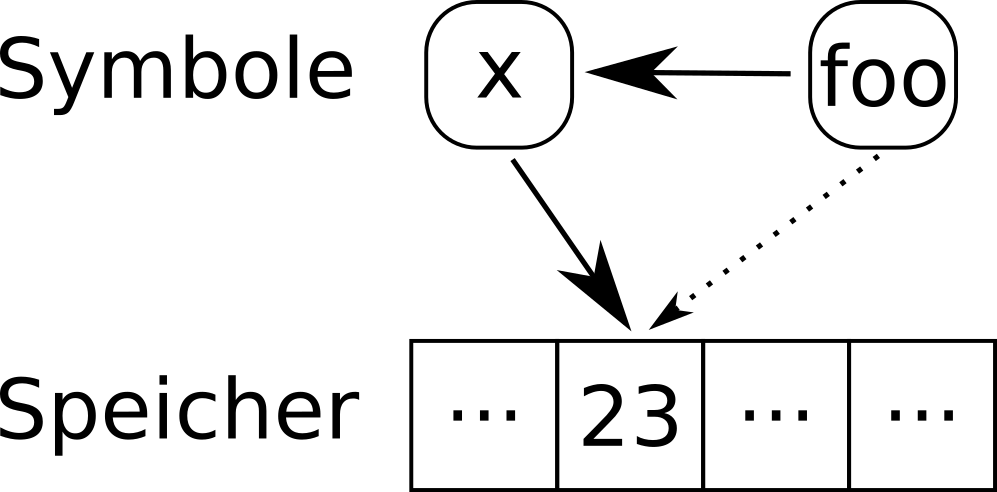
\includegraphics[width=.9\linewidth]{img/references.png}
\end{center}
\end{frame}
\begin{frame}[label={sec:org6b083b4},fragile]{Vergleich zwischen Zeiger und Referenz}
 \begin{minted}[numberblanklines=false,fontsize=\scriptsize]{c++}
// Erzeugen von Variable, Zeiger und Referenz
int intVar = 10;
int *intPtr = &intVar;
int &intRef = intVar;
// Auslesen von Variable, Zeiger und Referenz
cout << intVar << endl;
cout << *intPtr << endl;
cout << intRef << endl;
// Zuweisen an Variable, Zeiger und Referenz
intVar = 20;
*intPtr = 30;
intRef = 40;

cout << intVar << endl; // Ausgabe = 40
\end{minted}

Man sieht also, dass sich Referenzen genauso verwenden lassen wie
Variablen, aber zu großen Teilen die Funktionalität eines Zeigers
haben
\end{frame}
\begin{frame}[label={sec:org4b3b559}]{Referenzen als Parameter}
\begin{itemize}
\item Referenzen als Variablen in "normalem" Code sind eher unüblich
\item Referenzen werden am häufigsten bei Parametern von Funktionen
verwendet:
\begin{itemize}
\item Die übergebenen Parameter müssen dadurch nicht kopiert werden was
gerade bei großen Klassen schneller ist
\item Innerhalb der Funktion können Änderungen an den Parametern
vorgenommen werden welche auch ausserhalb der Funktion sichtbar
sind. Normalerweise funktioniert das nicht, weil die Änderungen
nur an einer Kopie vorgenommen werden.
\end{itemize}
\end{itemize}
\end{frame}
\begin{frame}[label={sec:org2e2c8f6},fragile]{Swap mit normalen Parametern, Zeigern, Referenzen}
 \begin{block}{Normale Parameter}
\begin{minted}[numberblanklines=false,fontsize=\scriptsize]{c++}
void swap(int p1, int p2) {
  int temp = p1; p1 = p2; p2 = temp;
}
int a = 2, b = 3; swap(a, b);   // Verwendung
\end{minted}
\footnotesize
Sieht einfach aus, funktioniert aber auch einfach nicht \ldots{}
\end{block}
\begin{block}{Zeiger}
\begin{minted}[numberblanklines=false,fontsize=\scriptsize]{c++}
void swap(int *p1, int *p2) {
    int temp = *p1; *p1 = *p2; *p2 = temp;
}
int a = 2, b = 3; swap(&a, &b); // Verwendung
\end{minted}
\end{block}
\begin{block}{Referenzen}
\begin{minted}[numberblanklines=false,fontsize=\scriptsize]{c++}
void swap(int &p1, int &p2) {
  int temp = p1; p1 = p2; p2 = temp;
}
int a = 2, b = 3; swap(a, b);  // Verwendung
\end{minted}
\end{block}
\end{frame}
\begin{frame}[label={sec:orga988b39}]{Swap -- Graphische Visualisierung}
\begin{center}
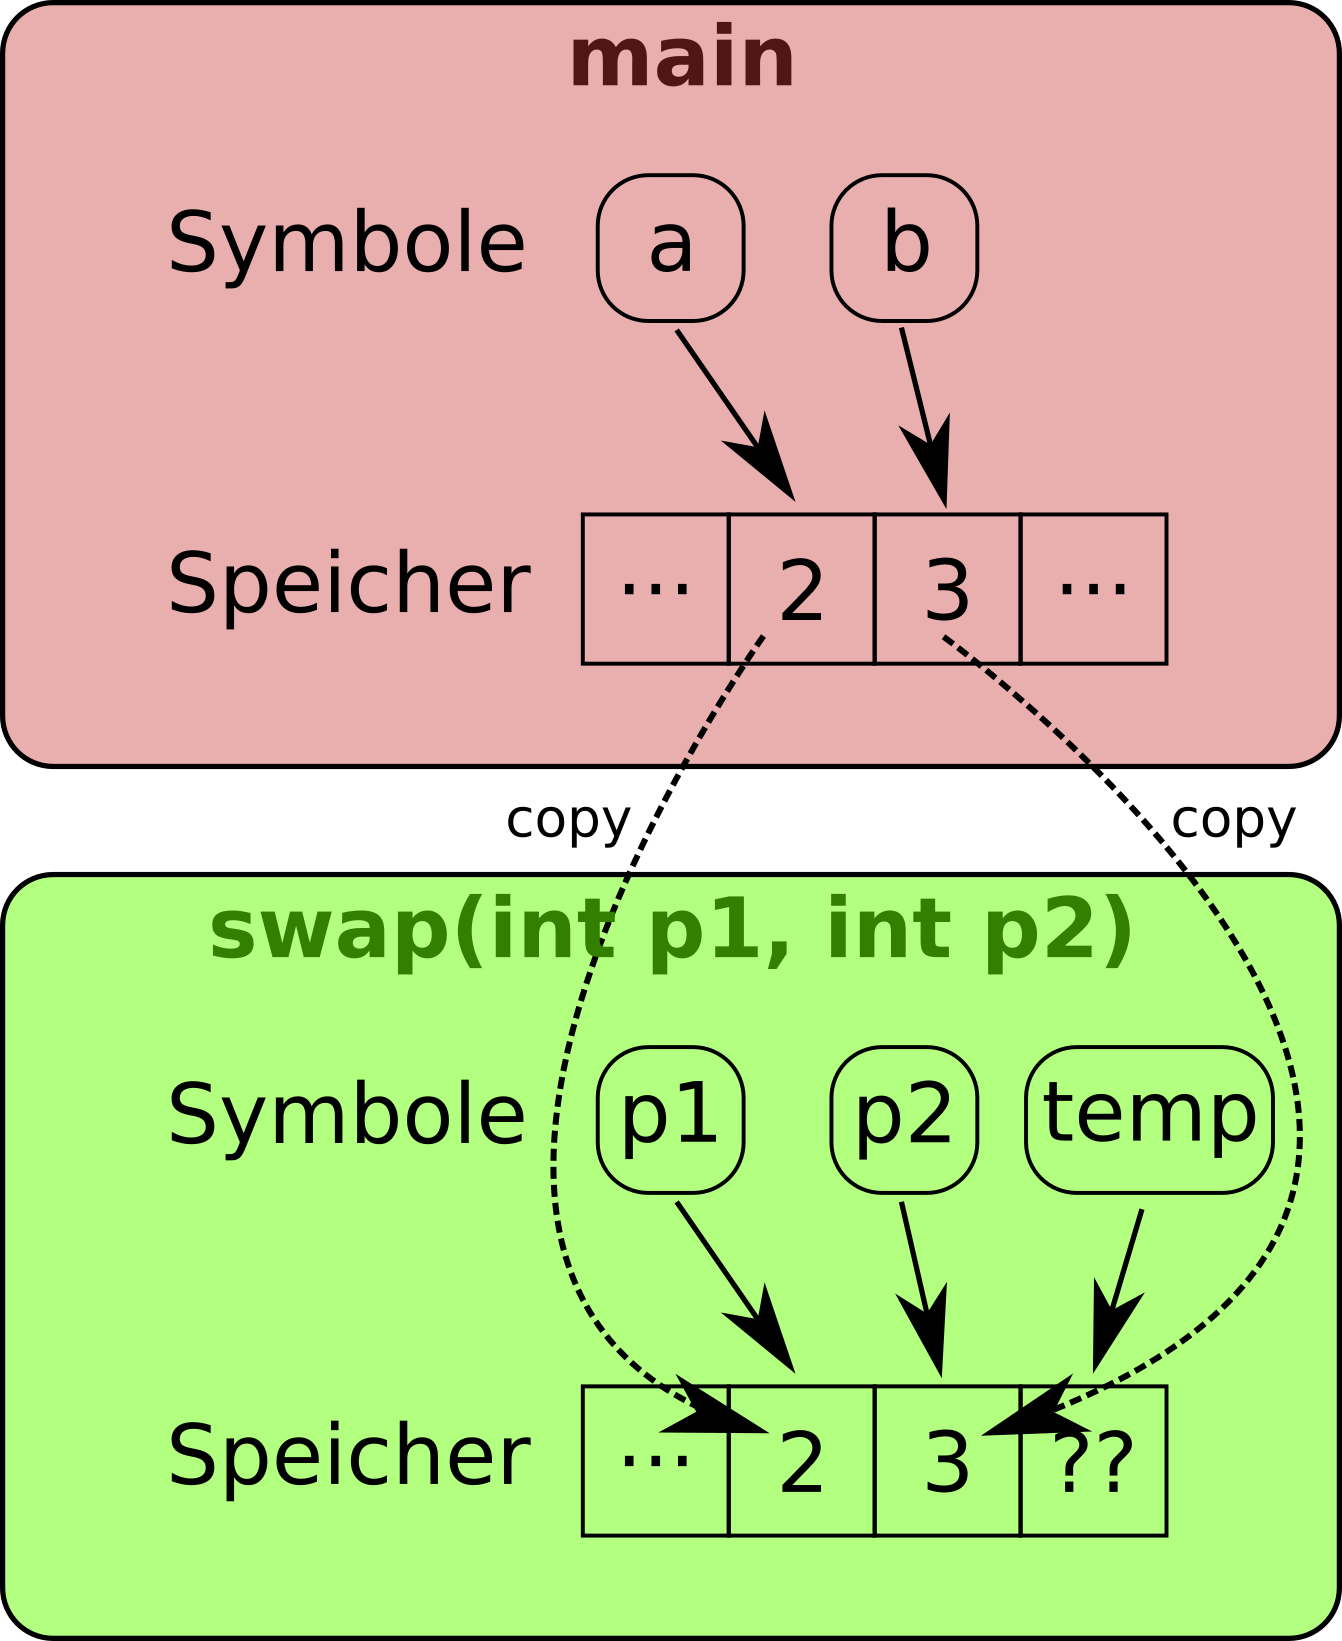
\includegraphics[width=0.6\textwidth]{img/swap_copy.png}
\end{center}
\end{frame}
\begin{frame}[label={sec:orgb83cafa}]{Swap -- Graphische Visualisierung}
\begin{center}
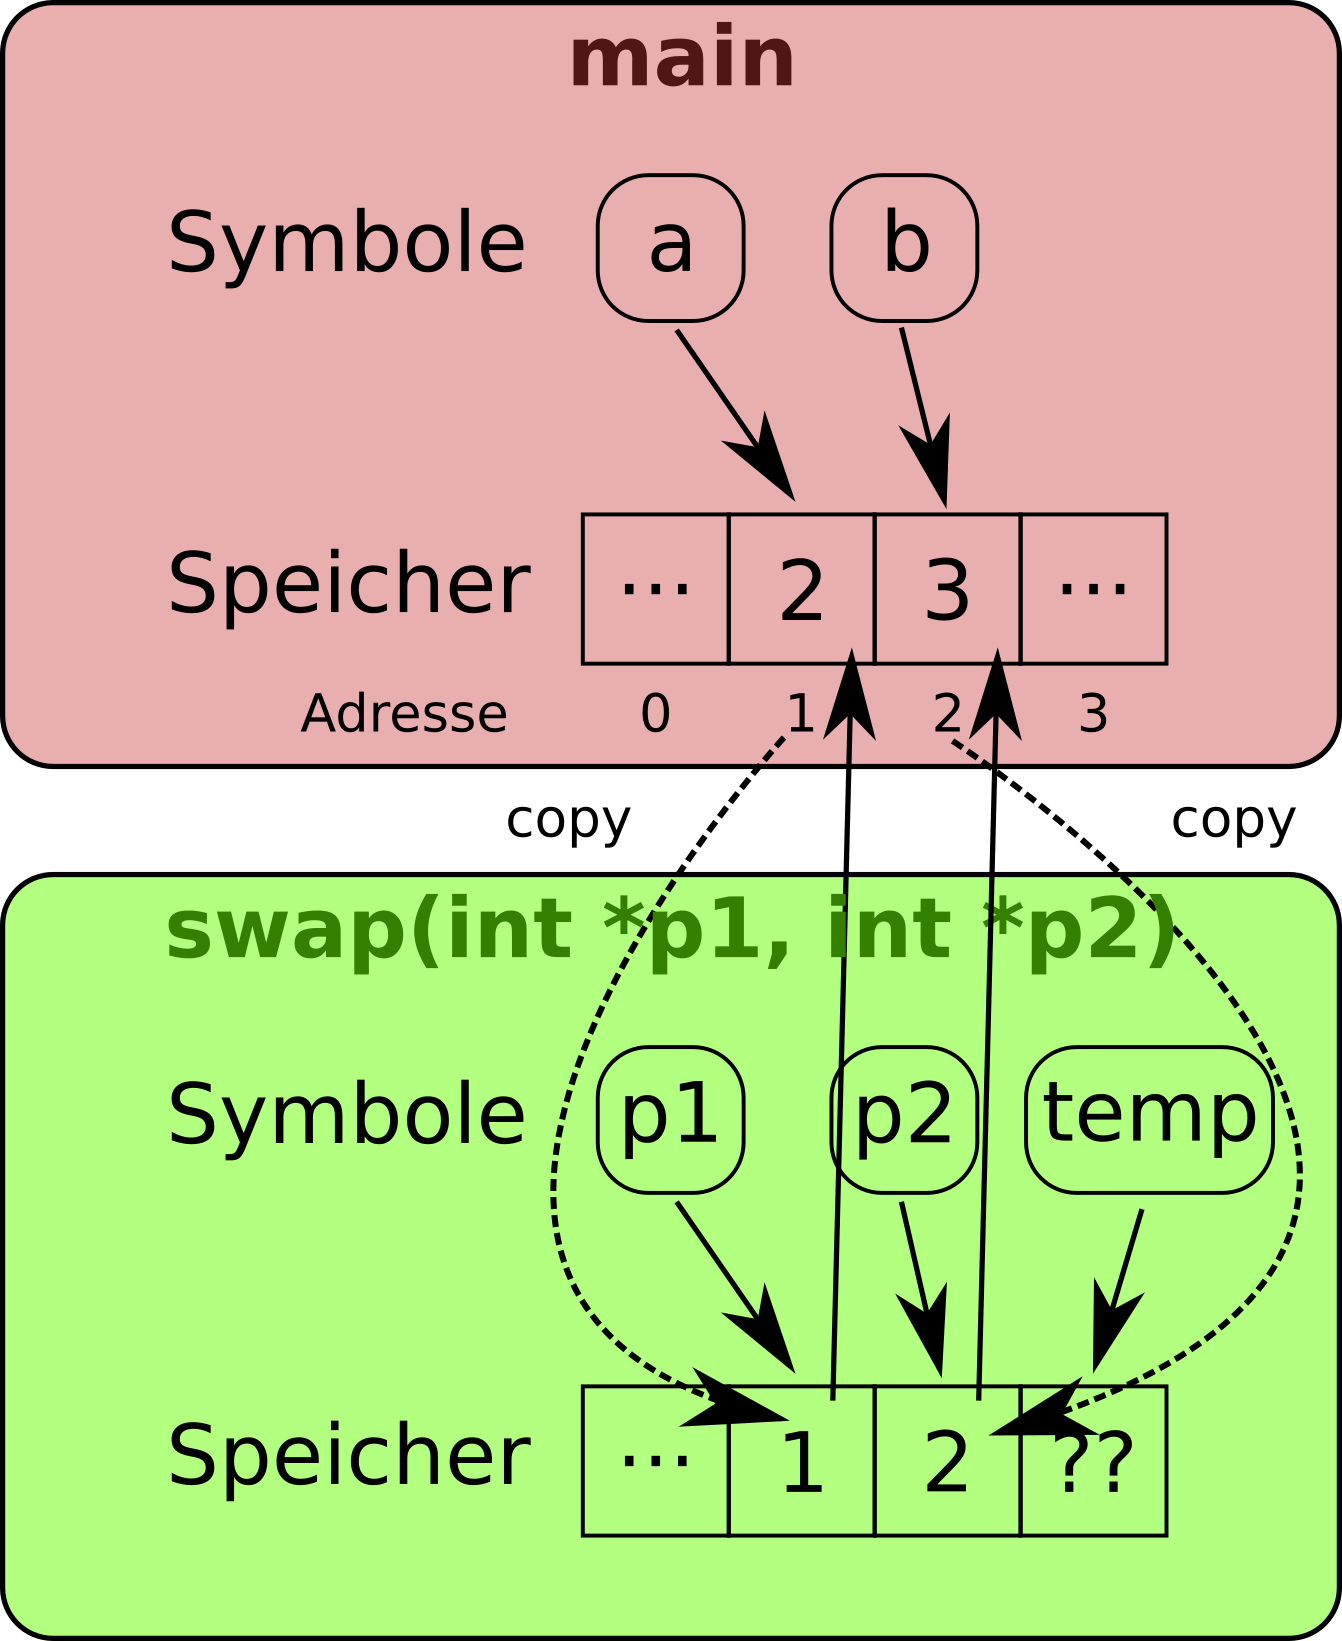
\includegraphics[width=0.6\textwidth]{img/swap_point.png}
\end{center}
\end{frame}
\begin{frame}[label={sec:org76537b7}]{Swap -- Graphische Visualisierung}
\begin{center}
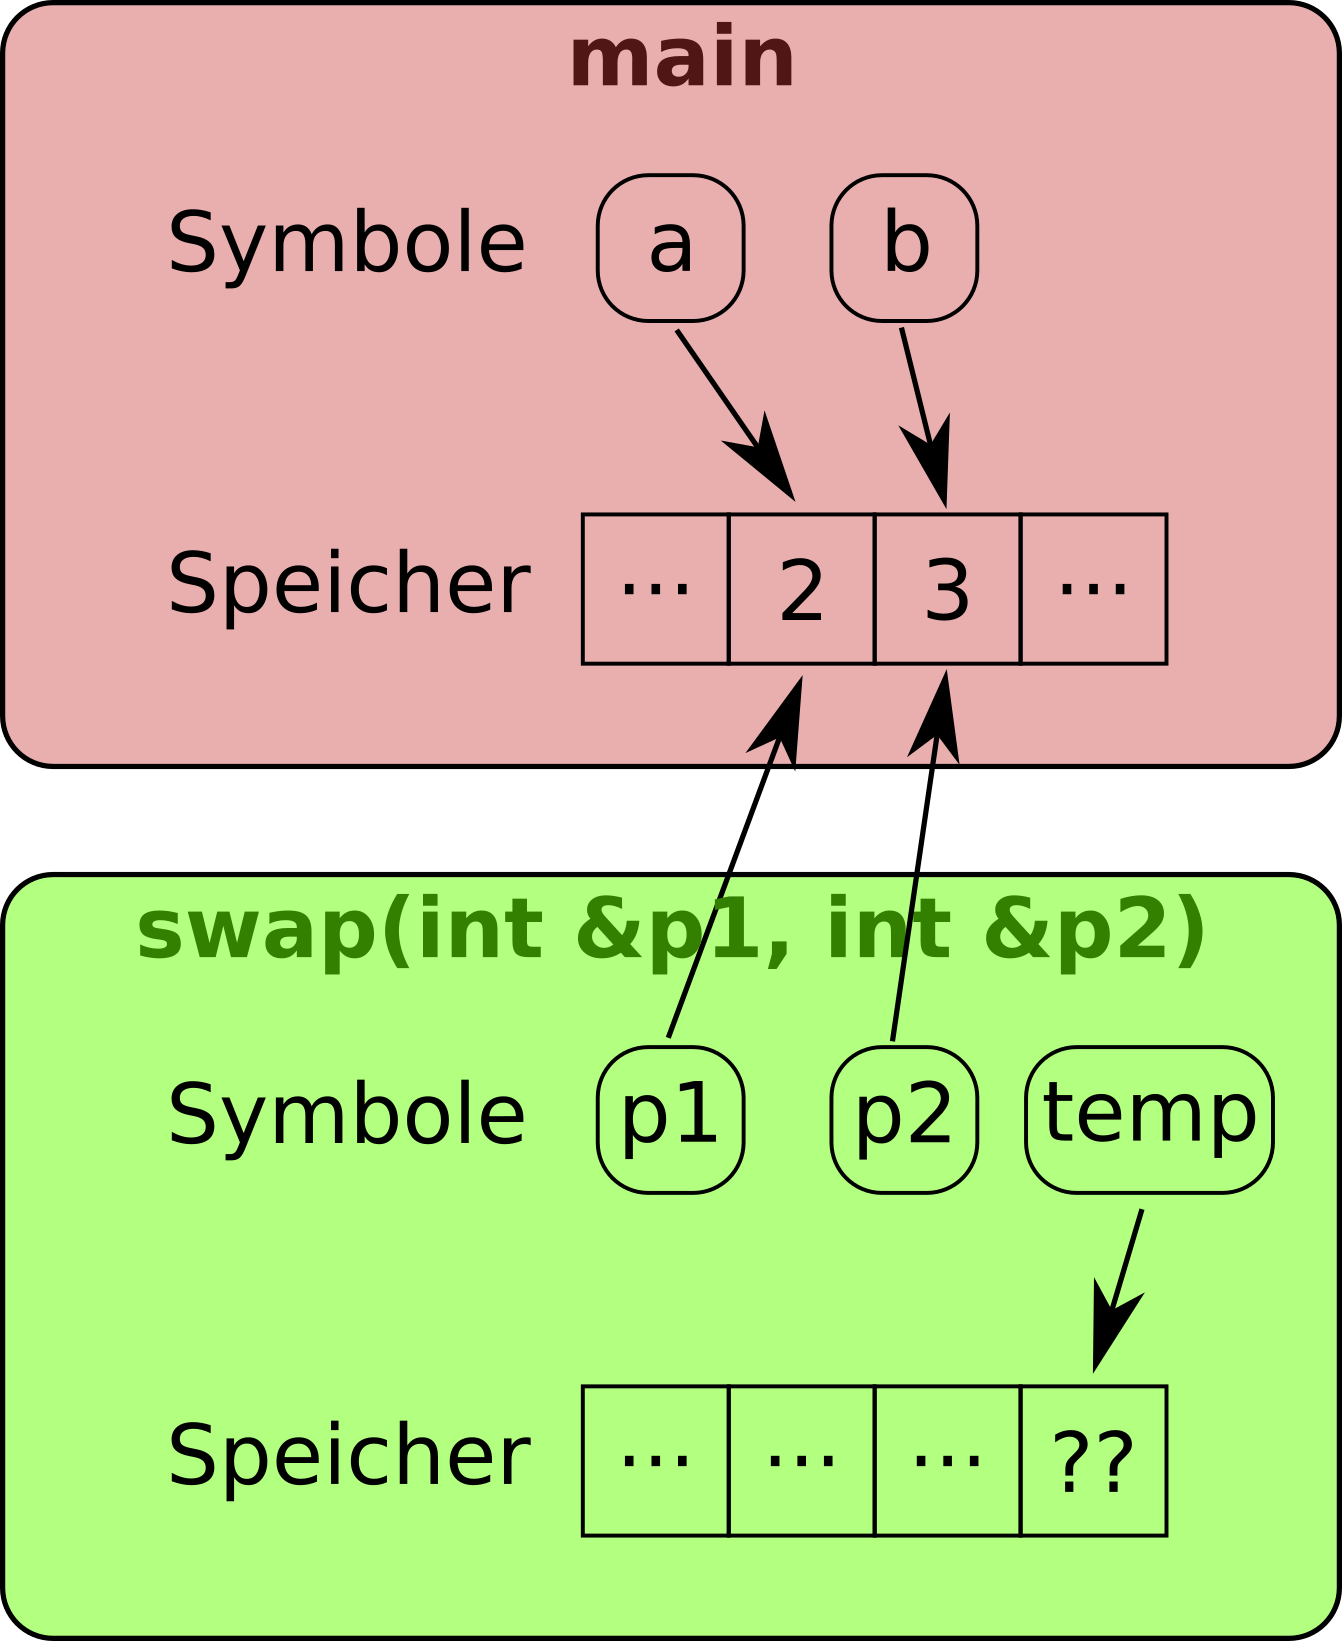
\includegraphics[width=0.6\textwidth]{img/swap_ref.png}
\end{center}
\end{frame}
\section{Casten}
\label{sec:org535d0d9}
\begin{frame}[label={sec:org40f7e52},fragile]{Casten "normaler" Datentypen}
 Casten einer "normalen" Variable konvertiert (so gut wie möglich) den
Inhalt einer Variable in einen anderen Datentyp
\begin{minted}[numberblanklines=false,fontsize=\scriptsize]{c++}
int i1 = 23;
double d1 = (double)i; // Konvertiert i explizit nach double
double d2 = 23.42;
int i2 = d2; // Hier wird implizit von double nach int konvertiert
\end{minted}
\end{frame}
\end{document}
